\documentclass[12pt]{report}
\usepackage{scribe,graphicx,graphics}


\course{MIT 22.213} 	
\coursetitle{Nuclear Reactor Kinetics}	
\semester{Spring 2015}
\lecturenumber{1}	
\lecturedate{}		


% Insert your name here!
\scribe{Geoffrey Gunow}

\begin{document}
	
	
	\maketitle
	
	\paragraph{Part A: Point Kinetics Equations}
	Using the point kinetics equations (PKE), the reactor power level $P$ can be computed as a function of time $t$ as a response to a varying reactivity $\rho(t)$ by solving the coupled equations:
	\begin{eqnarray}
	\frac{d}{dt} P(t) = \frac{\rho(t) - \sum_{i} \beta_i}{\Lambda} P(t) + \sum_{i} \lambda_i C_i(t) \label{eq1}\\
	\frac{d}{dt} C_i(t) = \frac{\beta_i}{\Lambda} P(t) - \lambda_i C_i(t) \label{eq2}
	\end{eqnarray}
	where for precursors in group $i$, $C_i$ denotes the precursor population, $\beta_i$ denotes the delayed neutron fraction, $\lambda_i$ denotes the time constant for the neutron emission, and the prompt neutron lifetime is given by $\Lambda$.
	
	These equations can be solved numerically by converting the equations into a linear algebra system of the form
	\begin{equation}
	\frac{d}{dt} N(t) = A N(t)
	\end{equation}
	where $N(t)$ is the solution vector encompassing reactor power levels and neutron precursor populations and $A$ is a matrix containing the appropriate combination of inputs ($\rho(t)$, $\beta_i$, $\lambda_i$, and $\Lambda$). A simple relation of the solution vector from one time step to another can be easily derived through the use of a matrix exponential:
	\begin{eqnarray}
		\frac{d}{dt} N(t) - A N(t) = 0 \\
		\frac{d}{dt} \left( N(t) e^{-At} \right) = 0 \\
		\int_{t' = t_{n-1}}^{t' = t_n} d\left(N(t') e^{-At'} \right) = \int_{t_{n-1}}^{t_n} 0 \, dt' \\
		N(t_n) e^{-At_n} - N(t_{n-1}) e^{-At_{n-1}} = 0 \\
		N(t_n) = N(t_{n-1}) e^{A(t_n - t_{n-1})} \\
		\boxed{N(t_n) = N(t_{n-1}) e^{A \Delta t}}
	\end{eqnarray}
	
	In addition to this equation, we need initial conditions for the solution vector. The initial power $P_0$ is calculated by
	\begin{equation}
	P_0 = \frac{W}{Q \Sigma_f}
	\end{equation}
	where $W$ is the power density, $Q$ is the energy released per fission, and $\Sigma_f$ is the averaged macroscopic fission cross-section. To calculate the initial precursor populations, we assume the system is initially in steady state. Using Eq.~\ref{eq2}, this yields the condition
	\begin{equation}
	C_{i,0} = \frac{P_0 \beta_i}{\Lambda \lambda_i}.
	\label{init_precursor}
	\end{equation}
	
	To solve the point kinetics equations, I implemented a modularized Python code with the use of numpy and scipy libraries which contain optimized solvers for such tasks as computing matrix exponentials. 
	
	\paragraph{Part B: Testing PKE Solver}
	Now we verify that our PKE solver is functioning correctly. First we need to ensure that the physical values we derive are correct. For example, we need to compute the total delayed neutron fraction. Editing the PKE solver yields $\boxed{ \beta = 0.006648}$.
	
	In addition, we need to calculate the prompt neutron lifetime, $\Lambda$. From the solver, $\boxed{\Lambda = 1.866386 \times 10^{-5}}$.
	
	Now to ensure the solver functions correctly, we need to show that it performs as expected when given a functional form of reactivity with time. In Fig.~\ref{pke}, the reactivity and reactor power are both plotted as a function of time. These results match the expected results given in the problem set.
	
	\begin{figure}[h!]
		\begin{center}
			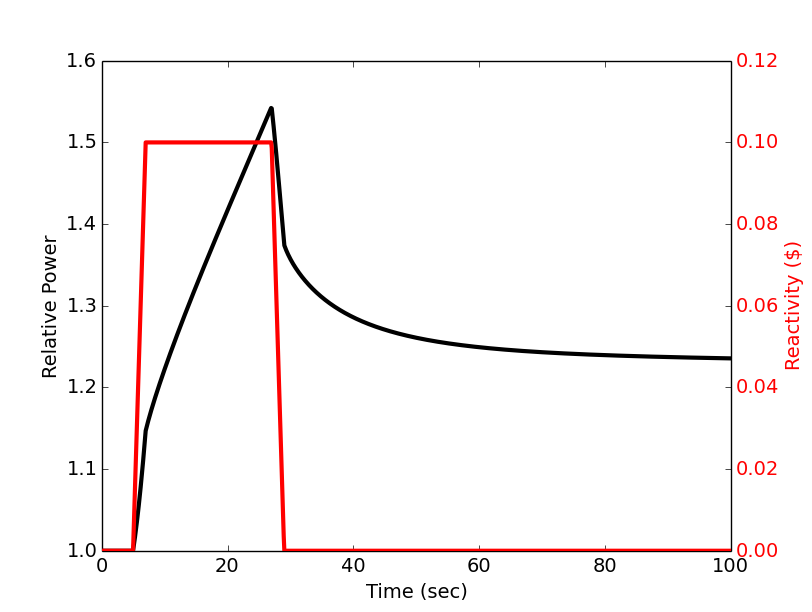
\includegraphics[scale=0.7]{partB.png}
		\end{center}
		\caption{Power level relative to initial value and reactivity in units of delayed neutron fractions (dollars) as a function of time.}
		\label{pke}
	\end{figure}
	
	In addition to the power level, it is also possible to plot precursor populations. The populations of each neutron precursor group are shown in Fig.~\ref{precursor}. We see that after the transient, the neutron precursor populations start to reach an equilibrium significantly greater than starting population. This explains why after the transient, the power level does not return to the original value. During the transient, the neutron precursor population is increased. When the reactor returns to critical the existence of more neutron precursors ensures that the equilibrium power level will be higher.
	
		\begin{figure}[h!]
			\begin{center}
				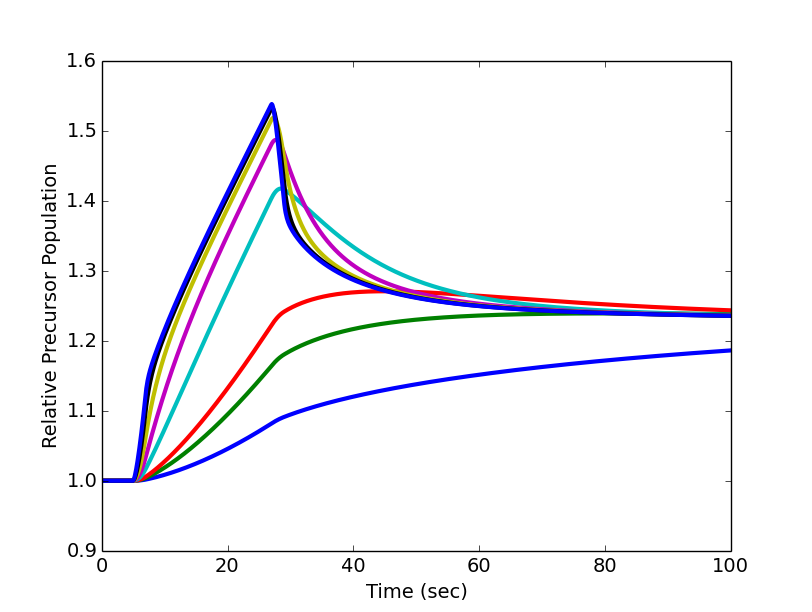
\includegraphics[scale=0.7]{partB_ex_precursors.png}
			\end{center}
			\caption{Neutron precursor populations relative to initial value as a function of time.}
			\label{precursor}
		\end{figure}
	
	\paragraph{Part C: Inverse Kinetics}
	Now we turn to the problem of inverse kinetics. This problems is very similar to the point kinetics problem except the desired reactor power as a function of time is given, and the reactivity required to produce the transient is calculated. 
	
	If we return to the original point kinetics equations, Eq.~\ref{eq1} can be rearranged as
	\begin{equation}
	\rho(t) = \frac{\Lambda}{P(t)} \frac{d}{dt} P(t) + \beta - \frac{\Lambda}{P(t)} \sum_i \lambda_i C_i(t). \label{eq_ike}
	\end{equation}
	Noting that the derivative of power can be approximated through finite difference if it is not available, the only further information needed is the precursor concentrations $C_i(t)$.
	
	If we return to Eq.~\ref{eq2}, we see that the precursor concentrations can be determined by solving simple ODEs when the power is known as a function of time. Therefore, the precursor populations can be derived through the use of an integrating factor:
	\begin{eqnarray}
	\frac{d}{dt} C_i(t) + \lambda_i C_i(t) = \frac{\beta_i}{\Lambda} P(t) \\
	\int_{t'=t_{n-1}}^{t'=t_n} d\left( C_i(t') e^{\lambda_i t'} \right) = \int_{t_{n-1}}^{t_n} \frac{\beta_i}{\Lambda} P(t') e^{\lambda_i t'} \, dt' \\
	C_i(t_n) e^{\lambda_i t_n} - C_i(t_{n-1}) e^{\lambda_i t_{n-1}} = \int_{t_{n-1}}^{t_n} \frac{\beta_i}{\Lambda} P(t') e^{\lambda_i t'} \, dt' \\
	C_i(t_n) =  C_i(t_{n-1})e^{-\lambda_i (t_n -t_{n-1})} + \frac{\beta_i}{\Lambda} \int_{t_{n-1}}^{t_n}  P(t') e^{\lambda_i (t_n - t')} \, dt'  \\
	C_i(t_n) =  C_i(t_{n-1})e^{-\lambda_i \Delta t} + \frac{\beta_i}{\Lambda} \int_{t_{n-1}}^{t_n}  P(t') e^{\lambda_i (t_n - t')} \, dt' 
	\end{eqnarray}
	
	Therefore, to solve for the precursor populations, we only need to attenuate the previous neutron population with the appropriate decay constant and add the neutron precursor production. The neutron precursor production is represented by the second term which can be solved with a simple quadrature.
	
	An alternative solution for precursor populations is presented in the lecture notes, which employs the use of matrix exponentials. However, the use of matrix exponentials adds unnecessary computational burden to the problem. Therefore, in the case where neutron precursor groups are independent given a known power profile (an assumption of the PKE equations), \textbf{matrix exponentials should not be used to compute the inverse kinetics solution}.
	
	Once we have calculated the precursor populations, Eq.~\ref{eq_ike} can be used with the backwards difference approximation to determine the reactivity as
	
	\begin{equation}
	\rho(t_n) = \frac{\Lambda}{P(t_n)}  \frac{P(t_n) - P(t_{n-1})}{\Delta t} + \beta - \frac{\Lambda}{P(t_n)} \sum_i \lambda_i C_i(t_n).
	\end{equation}
	
	Notice that we only need the initial precursor populations in addition to the power profile to calculate reactivity. For calculating the initial precursor populations, we use the same steady state assumption presented in Eq.~\ref{init_precursor} for the point kinetics solver.
	
	To verify that the solver is working correctly, the power profile calculated from the previous problem is input into the inverse kinetics solver. We should return the original profile. The result is presented in Fig.~\ref{ike1}.

	\begin{figure}[h!]
		\begin{center}
			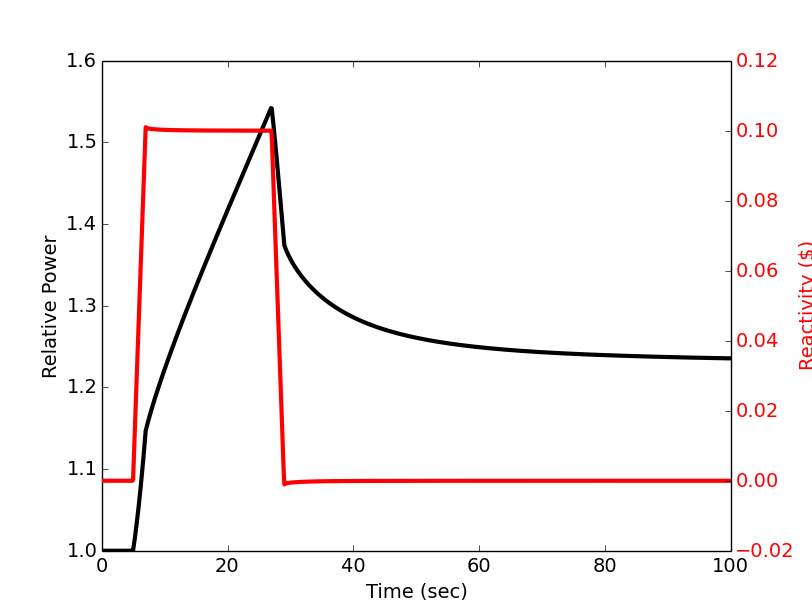
\includegraphics[scale=0.7]{partC_ex.png}
		\end{center}
		\caption{Inverse kinetics solution of reactivity profile using the calculated power profile presented in Fig.~\ref{pke}.}
		\label{ike1}
	\end{figure}
	 
	\newpage
	We see that the reactivity profile most nearly matches that given in part B. Slight discrepancies are noticed at sharp corners where the derivative is discontinuous, most likely due to difficulties in calculating the time derivative of power. In addition, it can be difficult to compute the quadrature of a function with discontinuities. 
	
	Finally, we test the inverse kinetics solver on a new transient. Our desired power shape involves an abrupt, discontinuous power increase by a factor of 100, holding a steady power for 8 seconds, followed a linear decline down to 10 times the original power. The result is presented in Fig.~\ref{ike2}.
	
	We see that a rapid increase in reactivity is required to boost the power to 100 times the initial power level. Then, the reactivity must decline so the power stays constant as the precursor populations grow. During the ramp decline, the reactivity plummets to lower the power and counteract the precursor growth. Once the desired power level is reached, the reactivity must once again increase to counteract the decline in precursor population.

	\begin{figure}[h!]
		\begin{center}
			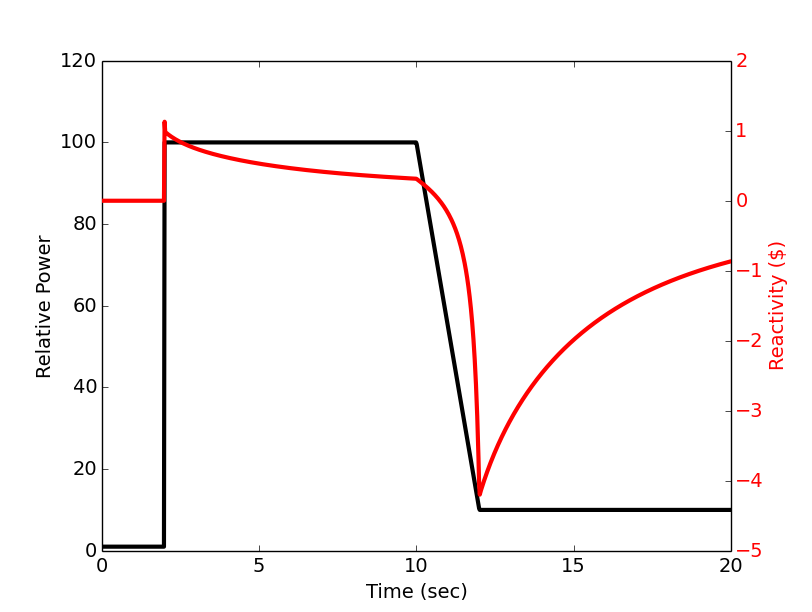
\includegraphics[scale=0.7]{partC.png}
		\end{center}
		\caption{Reactivity and power profiles as a function of time for the desired power profile presented in part C.}
		\label{ike2}
	\end{figure}
	
	

\end{document}